

\chapter{使用简介}
\label{chap:preplasmaEhancement}

\section{预脉冲与预等离子体}
\begin{figure}[!htbp]
  \centering
  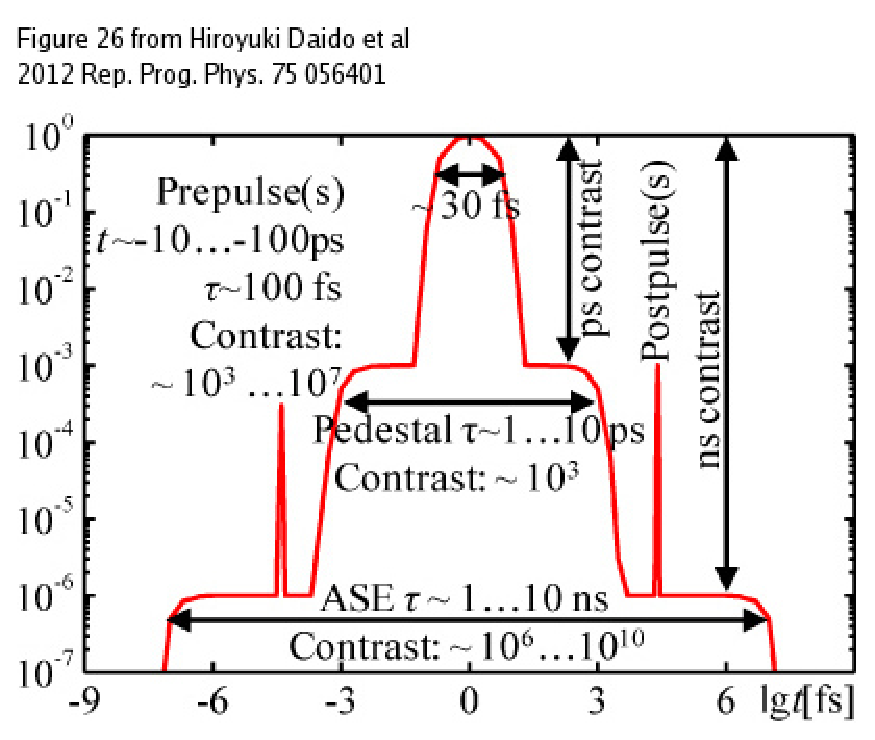
\includegraphics[width=\MyFactor\textwidth]{Img/prepulse2012.eps}
  \caption{激光脉冲示意图}
  \label{fig:prepulse2012}
\end{figure}

\begin{equation}
\label{eqn:freeStream}
q_{fs}=-n_e k T (k T / m_e)^{1/2}
\end{equation} 







上一章中,我们利用激光的预脉冲或者烧蚀脉冲产生预等离子体,而预等离子体的密度分布处于临界密度领域。临界密度我们已经做出定义,非相对论激光脉冲无法穿透。而当激光的光强到达相对论区域,由于相对论效应,等离子体频率相应的降低,因此激光穿透等离子体的能力增强。
当激光在等离子体中传播时,激光脉冲前沿的大部分电子被激光有质动力排开,形成通道结构,通道中由于电荷分离形成静电势,而通道中一部分电子在静电势中betatron震荡。另一方面,电子受到激光的驱动作用,当betatron震荡频率与激光频率匹配时,共振现象发生,电子能量吸收得到明显的增强,这种现象被称为DLA。A. Pukhov和J. Meyer-ter-Vehn对此有过很深入的研究,其研究结果表明,电子的温度相对于传统的有质动力加热有三倍以上的提高。


与此同时,在激光在等离子体传播的过程中,由于激光脉冲对于等离子体折射率的调制,会产生相对论自聚焦以及相对论相位自调制现象。相对论自聚焦现象使得激光的横向尺寸较小,相对论相位自调制使得激光的脉冲持续时间得到减小,最终结果使得激光的峰值光强得到明显的提高,同时激光的纵向分布得到整形,使得脉冲前沿更陡峭\cite{wanghongyong}。

在我们的研究中,希望使用预等离子体对于激光离子加速产生增强的作用。由于激光预脉冲可以有效地将激光能量转化给电子,而后通过电子传播至靶后,形成鞘层场加速离子,最终对于加速产生增强的作用。整个加速方案的模型,首先强度$10^{12}W/cm^2$,脉冲时间$100ps$量级烧蚀脉冲与$\mu m$量级的金属靶作用。通过调整烧蚀脉冲的持续时间,控制金属靶的烧蚀深度以及预等离子体膨胀,最终得到预等离子体与未烧蚀金属靶的双层靶结构。而后相对论强度的激光与双层靶作用,首先激光脉冲在临界密度的预等离子体中产生高能量高密度的DLA共振加热电子,接着共振电子传播至靶后面,在靶后建立起鞘层静电加速场。在这一模型的基础上,我们对于加速有如下的理论估计:
首先,加速的过程是在后表面由于电子产生的鞘层加速场产生的。因此仍然归类为TNSA加速机制。电子的加热的温度:

\begin{equation}
\label{eqn:DLAtemperature}
T_e = 1.8(I_{cpa} {\lambda}^2/{13.7}GW)^{1/2}
\end{equation} 



对比有质动力加热,其温度大约三倍或者以上,同时在聚焦磁场的作用下,电子束流得到聚焦压缩,密度得以提高。
对于加速时间,我们以fuchs的 $1.3 t_{laser}$的估计, 将以上估计带入到了绪论中关于激光加速TNSA理论中,粗略的估计可以得到,质子的能量增加至少三倍的结论。而其中的核心问题是电子的温度的提高的结果。


问题的集结点在于如何确保电子的温度可以达到最大值,而且保证高能量高密度的电子可以传播达到靶的后面。DLA电子高能高密,是由于共振效应,以及通道中磁场的聚焦效果的作用。因此电子能量密度,重要的条件是通道的存在,使得电子达到固体靶之前(因为固体靶中的电子由于相互之间的空间电荷力产生的密度减小可以忽略)仍然保持高度的聚焦状态。因此最有的加速条件:
激光在即将达到固体靶的时候耗尽所有的能量,此时DLA共振电子获得最大程度的能量增益,激光脉冲产生的通道有助于电子保持聚焦的高密度状态。
电子的加热和传输在很大程度上决定于等离子体的密度,而预等离子体的分布由预脉冲决定,因此可以通过控制预脉冲的参数,使得激光可以在即将达到固体靶时耗尽。对此我们有如下的估计:




